\documentclass[../modello-progetto.tex]{subfiles}

\begin{document}



\subsection{ Struttura dei file di AMPL}
\label{sub:struttura_dei_file_di_AMPL}

In allegato alla relazione verranno consegnati tre tipologie di file AMPL:
\begin{itemize}
	\item un file \textbf{.mod} che contiene la rappresentazione del modello illustrato precedentemente
	\item diversi file \textbf{.dat} che consentono il caricamento dei dati all'interno del modello
	\item un file \textbf{.run} necessario ad effettuare il caricamento del modello, dei dati e il reset in modalità automatica. Per il caricamento dei dati è necessario decommentare il file .dat che si vuole caricare nel modello.
\end{itemize}

\subsection{Risoluzione del problema}
\label{sub:risoluzione_del_problema}

Caricando il file \textit{modello.dat} ossia quello che rispecchia i dati del problema si può notare l'importanza del budget a disposizione del ristorante : un valore troppo basso di quest'ultimo infatti non riuscirà a soddisfare le richieste e quindi a pagare tutti i cuochi e il personale richiesto portando ad una soluzione impossibile. Allo stesso tempo un aumento minimo del budget a disposizione del ristorante incrementa in maniera sostanziale la qualità media della cena.

Con un budget di €35000 abbiamo il seguente risultato :
\begin{center}
	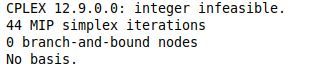
\includegraphics[width= 5cm]{img/35000-result.png}
\end{center}

Se proviamo ad approfondire il motivo per cui il problema risulta impossibile AMPL ci dirà quanto segue :
\begin{center}
	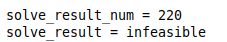
\includegraphics[width= 3cm]{img/35000-fault.png}
\end{center}
Un errore di tipo 200 indica, infatti, l'impossibilità di soddisfare tutti i vincoli contemporaneamente.

Solamente avendo un budget di circa €41000 (che è il budget del ristorante indicato nel testo del problema) AMPL riesce a trovare una soluzione ottima in 130 iterazioni :
\begin{center}
	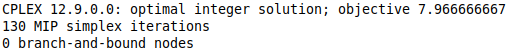
\includegraphics[width= 7cm]{img/41000-result.png}
\end{center}
Inoltre, è possibile osservare che il valore della funzione obiettivo aumenta quasi linearmente rispetto all'incremento di budget a disposizione del ristorante come nel grafico che segue:
\begin{center}
	\centering
	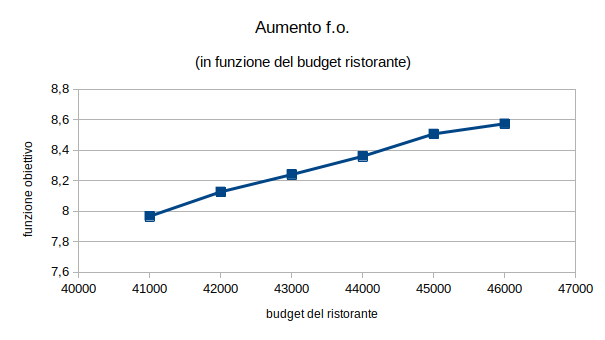
\includegraphics[width= 11cm]{img/grafico.png}
	\captionof{figure}{grafico che mostra l'aumentare della funzione obiettivo in concomitanza con l'incremento del budget del ristorante}
\end{center}

\subsection{Altri file .dat allegati}%
\label{sub:altri_.dat_allegati}

\paragraph{modello2.dat}%
\label{par:modello2.dat}

Il file modello2.dat presenta uno scenario leggermente diverso. Il ristorante ROItalia decide di organizzare una seconda cena di Gala dando la possibilità agli stessi cuochi della prima edizione di candidarsi. Tuttavia :
\begin{itemize}
	\item I cuochi M ed O decidono di non ricandidarsi.
	\item La complessità dei cibi è cambiata, infatti sono ora richiesti 3 cuochi per realizzare antipasto e dessert, 2 per primo piatto e secondo e 4 per secondo primo piatto.
	\item Il budget del ristorante è di €54000.
	\item Il numero massimo di portate realizzabili per ciascun cuoco è 3 invece che 2. Tuttavia, un cuoco può ancora realizzare una portata aggiuntiva ottenendo un surplus di €1200.
	\item Il costo di un cameriere è €1100 mentre il costo di un aiuto cuoco è di €700.
\end{itemize}

\paragraph{modello3.dat}
\label{par:modello3.dat}

Il file modello3.dat rappresenta la terza cena di Gala organizzata dal ristorante ROItalia. Per la terza edizione si è deciso di assumere cuochi che non avevano mai partecipato alle edizioni precedenti. Tuttavia, anche in questa occasione sarà necessario effettuare una prova per stabilire chi cucinerà. Inoltre, il budget a disposizione del ristorante è questa volta assai più alto e pari a €50000. Per questa ragione si è deciso di attribuire un compenso maggiore ad ogni cuoco e sempre sulla base del voto medio ottenuto svolgendo le cinque prove. La tabella sottostante mostra il compenso promesso:

\begin{center}
	\begin{tabular}{p{3cm} | p{4cm}}
	\hline
	fascia & compenso(in euro) \\
	\hline
	\hline
	5 \leq media \leq 6 & 1000 \leq prezzo \leq 1400 \\
	6 \leq media \leq 7 & 1900 \leq prezzo \leq 2300 \\
	7 \leq media \leq 8 & 2600 \leq prezzo \leq 3000 \\
	8 \leq media \leq 9 & 3300 \leq prezzo \leq 3700\\
	9 \leq media \leq 10 & 4000\leq prezzo \leq 4400\\
	\hline
	\end{tabular}
\end{center}
Inoltre, si deve considerare che :
\begin{itemize}
	\item il costo di un cameriere è €950 mentre il costo di un aiuto cuoco è €750.
	\item Sono necessari 3 cuochi per ogni portata.
	\item Un cuoco può realizzare al più 3 portate.
	\item Il surplus che deve essere dato al cuoco che eventualmente cucinerà la quarta portata è di €2000.
\end{itemize}
\end{document}